\chapter[Referencial Teórico]{Referencial Teórico}

\section{Débito Técnico}
Débito técnico é uma metáfora proposta por \cite{cunningham} onde, uma dívida é
criada quando a qualidade do código é deixada de lado para acelerar o processo
de desenvolvimento, até o momento que esta dívida é quitada. O preço do pagamento
da dívida, geralmente feita através de refatoração,  aumenta gradualmente com
a evolução do projeto.

\cite{oliveira} afirma que se pode identificar vários atributos em um Débito
Técnico, sendo eles:

\begin{itemize}
  \item Reason, motivo pelo qual o débito foi adquirido;
  \item Benefíts, o lucro ou ponto positivo que a escolha de optar pelo débito traz;
  \item Result, o que esse débito realmente possibilitou para a organização;
  \item Principal, representa o preço que o pagamento do débito possui no momento;
  \item Interest, preço de pagamento do débito depois de um dado tempo;
  \item Returns, quanto a organização lucrou com a decisão de ter optado pelo Débito Técnico.
\end{itemize}


De acordo com \cite{mapping}, há um debate sobre a importância de gerenciar o
Débito Técnico, pois este é muito importante para a equipe de negócios,
complementando que nem sempre este é ruim, e que podem trazer benefícios
que são maiores do que a perca monetária causada pelo juros.

\cite{mapping} identificam que o Débito Técnico tem atividades que podem ser classificadas.
Ela lista oito tipos de Débito Técnico, sendo eles:

\begin{itemize}
  \item Identificação;
  \item Medição;
  \item Priorização;
  \item Prevenção;
  \item Monitoramento;
  \item Pagamento;
  \item Representação/Documentação;
  \item Comunicação;
\end{itemize}

Quando se trata de Débito Técnico, existem modelos de identificação e medição de
código. O autor \cite{eisenberg}, executa uma análise estática e utiliza o
resultado para estimar o quanto custará para sanar todo ou parte do Débito
Técnico existente em um projeto.



\subsection{Método SQALE para avaliação de Débito Técnico}
\cite{letouzey} propõe a utilização do método SQALE (Software Quality Assessment
based on Lifecycle Expectations) para análise do débito técnico. O método de
Letouzey propõe um Modelo de Qualidade (SQALE Quality Model) e um Modelo de
Análise (SQALE Analysis Model) para verificação das violações de código.

O Modelo de Qualidade do SQALE constitui de uma matriz hierárquica de 3 níveis:
Características, Sub-Caracteristicas e Requisitos. Numa estratégia de análise de
débito técnico, pode ser definido que qualquer não-conformidade do código com os
requisitos caracteriza débito técnico. Por isso, os Requisitos devem ser atômicos,
não-ambíguos, não-redundantes, justificáveis, aceitáveis, implementáveis e
verificáveis.

Assim, basta utilizar uma ferramenta que consiga avaliar o código com relação
aos Requisitos estabelecidos e será possível identificar o débito técnico na
aplicação.

O Modelo de Análise faz uso de um índice de remediação para avaliar os
impactos das violações identificadas. Esse índice de remediação faz uma relação
entre os Requisitos do Modelo de Qualidade, com uma remediação associada a
cada violação desses requisitos. Por fim, é estipulado também uma função de
remediação, que associa um tempo para aplicar aquela remediação.

\subsection{Identificação de Débito Técnico}
Para mensurar o Débito Técnico existente em uma aplicação é necessário que haja
meios de identificá-lo. Existem vários métodos de identificação de Débito Técnico,
sendo um deles o proposto por \cite{siebra}, afirmando que os resultados obtidos a
partir da medição de um conjunto de dez métricas podem identificar o quanto de
Débito Técnico uma aplicação possui. Essas métricas podem ser:

\begin{enumerate}
  \item Acoplamentos Aferentes;
  \item Acoplamentos Eferentes;
  \item Árvore de Profundidade de Herança;
  \item Falta de Coesão em Métodos;
  \item Número de filhos;
  \item Complexidade Cliclomática;
  \item Duplicação de Código;
  \item Documentação do Código;
  \item Métodos por classe;
  \item Acoplamento entre métodos.
\end{enumerate}

\subsection{Medição de Débito Técnico}
\cite{principal} propõem uma fórmula para identificação do principal de um
débito técnico, com parâmetros ajustáveis de acordo com os interesses da
organização. A formula é:

\begin{figure}[h]
  \centering
  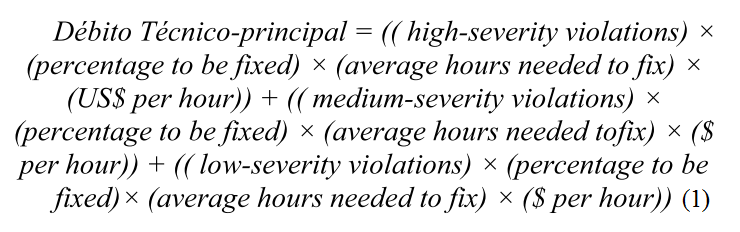
\includegraphics[width=250px, scale=1]{figuras/formulaprincipal}
  \caption{Cálculo do TD principal}
\end{figure}
Onde:

Débito Técnico-Principal: É o valor atual de Débito Técnico no software;

X-Severity-Violations: O somatório total de números de ocorrências de violações
de uma severidade X;

Percentage to be fixed: O percentual que a organização estipulou que irá corrigir
de violações daquele nível de severidade;

Average hours needed to fix: Média do tempo necessário para corrigir uma violação
daquele nível de severidade;

\$ per hour: Custo/hora de quem irá corrigir as violações.

Segundo os autores, com a fórmula é possível obter o custo para corrigir o débito
técnico de um software, de acordo com os parâmetros da organização.

\section{Contratação na Administração Pública Federal Brasileira}

No Decreto-Lei nº 200, \cite{decreto200} por institui princípios fundamentais para a
Administração Pública, sendo um deles a contratação de terceiros, que deve ser
executada sempre que houver possibilidade.

O decreto nº 2.271, por \cite{decreto2271}, aconselha que todos os produtos e seviços
que não tenham ligação direta para a utilização na organização, incluindo serviços
de informática, sejam terceirizados. A fim de destituir a responsabilidade do
órgão para com o desenvolvimento de vários serviços, privando-o unicamente com
a administração destes.

\section{Medição e Análise}
\subsection{GQM}
